\section{Results}

The system was implemented as described in the previous sections.
It was tested by applying a step function of 1.89 N, and recording the system response.
The resulting magnet position can be seen in figure \ref{fig:position} and its velocity in \ref{fig:velocity}.
Observer results are also presented in this graph.

\begin{figure}[p]
    \centering
    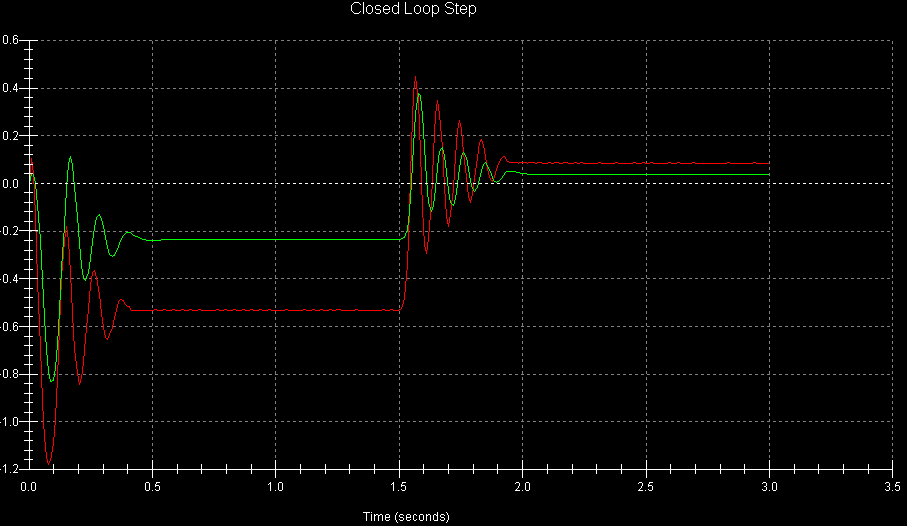
\includegraphics[width=1\textwidth]{position}
    \caption{System Response: Position - Actual (Red) and Observed (Green)}
    \label{fig:position}
\end{figure}

\begin{figure}[p]
    \centering
    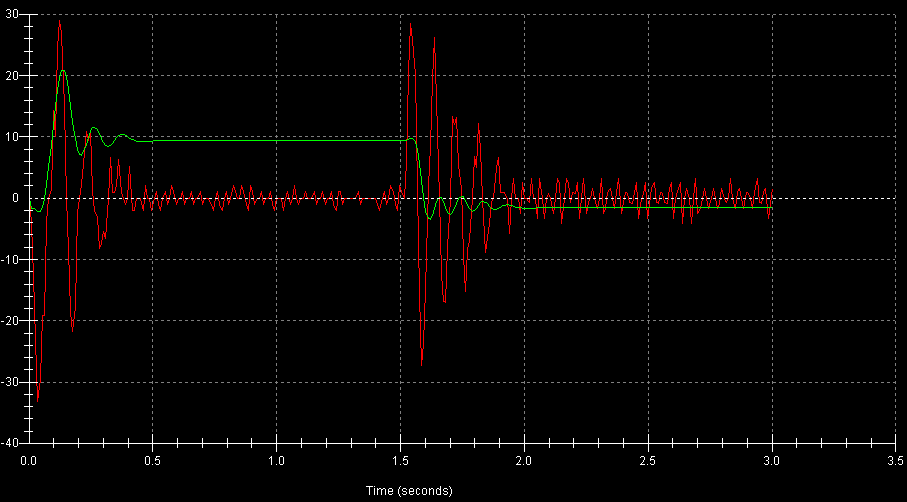
\includegraphics[width=1\textwidth]{velocity}
    \caption{System Response: Velocity - Actual (Red) and Observed (Green)}
    \label{fig:velocity}
\end{figure}
